\section{nonlinear least squares}

\label{sec:6.2}

Let's consider a simple least squares problem first:

\begin{equation}
\mathop {\min }\limits_{\bm{x}} F(\bm{x}) = \frac{1}{2}{\left\| {f\left( \bm{x} \right)} \right\|^2_2}.
\end{equation}

Where the argument $\bm{x} \in \mathbb{R}^n$, $f$ is an arbitrary scalar nonlinear function $f(\bm{x}): \mathbb{R}^n \mapsto \ Mathbb{R}$. Note that the coefficient $\frac{1}{2}$ is irrelevant. Some documents have this coefficient, and some documents do not. It does not affect the subsequent conclusions. Let's discuss how to solve such an optimization problem. Obviously, if $f$ is a mathematically simple function, then the problem can be solved in analytical form. Let the derivative of the objective function be zero, and then solve the optimal value of $\bm{x}$, just like the extreme value of the binary function:

\begin{equation}
\frac{ \mathrm{d} F}{ \mathrm{d} \bm{x} } = \bm{0}.
\end{equation}

Solving this equation yields an extremum with a derivative of zero. They may be maximal, very small, or values at the saddle point, as long as they compare the size of their function values one by on. But is this equation easy to solve? This depends on the form of the $f$ derivative. If $f$ is a simple linear function, then the problem is a simple linear least squares problem, but some derivatives may be complex in form, making the equation not easy to solve. Solving this equation requires us to know the \textbf{global nature} of the objective function, which is usually not possible. For the least squares problem that is inconvenient to solve directly, we can use the \textbf{iteration} method to continuously update the current optimization variable from an initial value to make the objective function drop. The specific steps can be listed as follows:

\begin{mdframed}  
	\begin{enumerate}
		\item gives an initial value of $\bm{x}_0$.
		\item For the $k$ iteration, look for an increment of $\Delta \bm{x}_k$, making $\left\| {f\left( \bm{x}_k + \Delta \bm{x} _k \right)} \right \|^2_2$ reaches a minimum value.
		\item Stop if $\Delta \bm{x}_k$ is small enough.
		\item Otherwise, let $\bm{x}_{k+1} = \bm{x}_k+\Delta \bm{x}_k$ return to step 2.
	\end{enumerate}
\end{mdframed}

This turns the problem of solving the \textbf{The derivative function is zero} The problem has become a constant \textbf{find drop increment} $\Delta \bm{x}_k$ problem, as we will see, since it can be $f$ Linearization, the calculation of the increment will be much simpler. When the function drops until the increment is very small, the algorithm is considered to converge and the objective function reaches a minimum value. In this process, the problem is how to find the increment of each iteration point, and this is a local problem, we only need to care about the local nature of $f$ at the iteration value rather than the global nature. Such methods are widely used in areas such as optimization and machine learning.
	
Next we look at how to find this increment $\Delta \bm{x}_k$. This part of the knowledge is actually in the field of numerical optimization, let's look at some widely used results.

\subsection{Basic use of Sophus}

We have introduced the introductory knowledge of Lie algebra, and now it is time to consolidate what we have learned through practical exercises. Let's discuss how to manipulate Lie algebra in a program. In Lecture 3, we saw that Eigen provided geometry modules, but did not provide support for Lie algebra. A better Lie algebra library is the Sophus library maintained by Strasdat\footnote{The earliest proposed Lie algebra is Sophus Lie, which is named after him. }. The Sophus library supports $\mathrm{SO}(3)$ and $\mathrm{SE}(3)$, which are mainly discussed in this chapter. In addition, it also contains two-dimensional motion $\mathrm{SO}(2), \mathrm{SE} (2) $ and the similar transformation of $\mathrm{Sim}(3)$. It is developed directly on top of Eigen and we don't need to install additional dependencies. Readers can get Sophus directly from GitHub, or the Sophus source code is also available in the book's code directory slambook/3rdparty. For historical reasons, earlier versions of Sophus only provided double-precision Lie group/Lie algebra classes. Subsequent versions have been rewritten as template classes. Different precision Lie group/Lie algebra can be used in the Sophus of the template class, but at the same time it increases the difficulty of use. In the second edition of this book, we use the Sophus library of \textbf{with template}. The Sophus provided in the 3rdparty of this book is the \textbf{template} version, which should have been copied when you downloaded the code for this book. Sophus itself is also a cmake project. Presumably you already know how to compile the cmake project, so I won't go into details here. The Sophus library only needs to be compiled, no need to install it.

Let's demonstrate the SO(3) and SE(3) operations in the Sophus library:

\begin{lstlisting}[language=c++,caption=slambook/ch4/useSophus.cpp]
#include <iostream>
#include <cmath>
#include <Eigen/Core>
#include <Eigen/Geometry>
#include "sophus/se3.hpp"

Using namespace std;
Using namespace Eigen;

/// This program demonstrates the basic usage of sophus
Int main(int argc, char **argv) {
// Rotation matrix rotated 90 degrees along the Z axis
Matrix3d R = AngleAxisd(M_PI / 2, Vector3d(0, 0, 1)).toRotationMatrix();
// or quaternion
Quaterniond q(R);
Sophus::SO3d SO3_R(R); // Sophus::SO3d can be constructed directly from the rotation matrix
Sophus::SO3d SO3_q(q); // can also be constructed by quaternion
// Both are equivalent
Cout << "SO(3) from matrix:\n" << SO3_R.matrix() << endl;
Cout << "SO(3) from quaternion:\n" << SO3_q.matrix() << endl;
Cout << "they are equal" << endl;

// Use the logarithmic map to get its Lie algebra
Vector3d so3 = SO3_R.log();
Cout << "so3 = " << so3.transpose() << endl;
// hat is vector to antisymmetric matrix
Cout << "so3 hat=\n" << Sophus::SO3d::hat(so3) << endl;
// Relative, vee is the objection vector
Cout << "so3 hat vee= " << Sophus::SO3d::vee(Sophus::SO3d::hat(so3)).transpose() << endl;

// Update of the incremental disturbance model
Vector3d update_so3(1e-4, 0, 0); //assuming the update is so much
Sophus::SO3d SO3_updated = Sophus::SO3d::exp(update_so3) * SO3_R;
Cout << "SO3 updated = \n" << SO3_updated.matrix() << endl;

Cout << "*******************************" << endl;
// The same is true for SE(3) operations
Vector3d t(1, 0, 0); // translate 1 along the x axis
Sophus::SE3d SE3_Rt(R, t); // Construct SE(3) from R, t
Sophus::SE3d SE3_qt(q, t); // Construct SE(3) from q,t
Cout << "SE3 from R,t= \n" << SE3_Rt.matrix() << endl;
Cout << "SE3 from q,t= \n" << SE3_qt.matrix() << endl;
// The Lie algebra se(3) is a six-dimensional vector. For convenience, typedef is used first.
Typedef Eigen::Matrix<double, 6, 1> Vector6d;
Vector6d se3 = SE3_Rt.log();
Cout << "se3 = " << se3.transpose() << endl;
// Observe the output, you will find that in Sophus, the translation of se(3) is in front and the rotation is in the back.
// Same, there are two operators of hat and vee
Cout << "se3 hat = \n" << Sophus::SE3d::hat(se3) << endl;
Cout << "se3 hat vee = " << Sophus::SE3d::vee(Sophus::SE3d::hat(se3)).transpose() << endl;

// Finally, demonstrate the update
Vector6d update_se3; //update volume
update_se3.setZero();
Update_se3(0, 0) = 1e-4d;
Sophus::SE3d SE3_updated = Sophus::SE3d::exp(update_se3) * SE3_Rt;
Cout << "SE3 updated = " << endl << SE3_updated.matrix() << endl;

Return 0;
}
\end{lstlisting}

The demo is divided into two parts. The first half introduces the operation on $\mathrm{SO}(3)$, and the second half is $\mathrm{SE}(3)$. We demonstrate how to construct $\mathrm{SO}(3), \mathrm{SE}(3)$ objects, exponentially, logarithmically map them, and update the lie group elements when we know the update amount. If the reader has a good understanding of the content of this lecture, then this program should not be difficult for you. In order to compile it, add the following lines to CMakeLists.txt:

\begin{lstlisting}[caption=slambook/ch4/useSophus/CMakeLists.txt]
# To use sophus, you need to find it using the find_package command
Find_package( Sophus REQUIRED )
Include_directories( ${Sophus_INCLUDE_DIRS} )

Add_executable( useSophus useSophus.cpp )
\end{lstlisting}

The find\_package command is an instruction provided by cmake to find the header and library files of a library. If cmake can find it, it will provide the variables for the directory where the header and library files are located. In the example of Sophus, it is Sophus\_INCLUDE\_DIRS. The template-based Sophus library, like Eigen, contains only header files and no source files. Based on them, we can introduce the Sophus library into our own cmake project. Readers are asked to see the output of this program on their own, which is consistent with our previous derivation.


\subsection{Euclidean transformation between coordinate systems}
We often define a variety of coordinate systems in the actual scene. In robotics, you define each coordinate system for each link and joint; in 3D mapping, we also define the coordinate system for each cuboid and cylinder. If you consider a moving robot, it is common practice to set an inertial coordinate system (or world coordinate system) that can be considered stationary, such as 
$ \bm{TODO(Hussein)} $ defined coordinate system. At the same time, the camera or robot is a moving coordinate system, such as the coordinate system defined by $x_C, y_C, z_C$. We might ask: a vector $\bm{p}$ in the camera's field of view, with coordinates in the camera coordinate system of $\bm{p}_c$, and in the world coordinate system, its coordinates are $ \bm{p}_w$, then how is the conversion between these two coordinates? At this time, it is necessary to first obtain the coordinate value of the point for the robot coordinate system, and then according to the robot pose \textbf{transform} into the world coordinate system. We need a mathematical means to describe this transformation. As we will see later, we can describe it with a matrix $\bm{T}$.

\begin{figure}[!htp]
	\centering
  	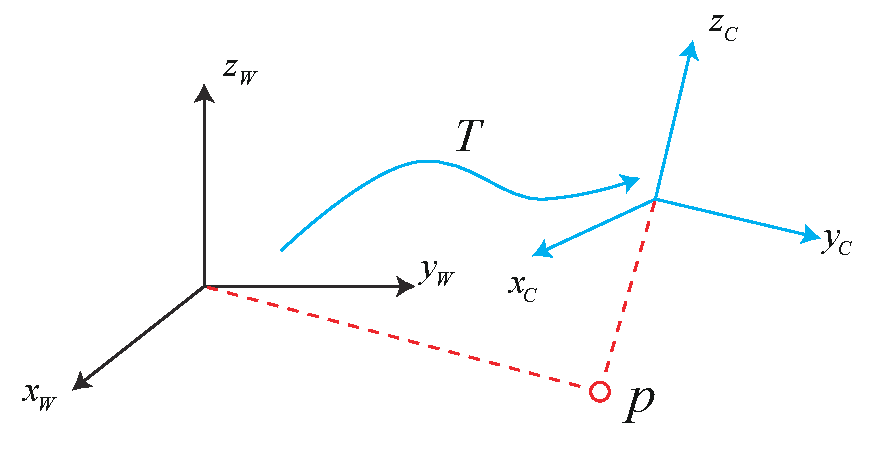
\includegraphics[width=0.7\textwidth]{chapter03/rigidMotion/axisTransform.pdf}
	\caption {Coordinate transformation. For the same vector $ \bm{} the p- $ , it coordinates in the world coordinate system $ \bm{} _w the p- $ and coordinate in the camera coordinate system $ \bm{} _c the p- $ is different. This transformation relationship is described by the transformation matrix $ \bm{T} $ . }
	\label{fig:axisTransform}
\end{figure}

Intuitively, the motion between two coordinate systems consists of a rotation plus a translation called \textbf {rigid body motion}. Camera movement is a rigid body movement. During the rigid body motion, the length and angle of the same vector in each coordinate system will not change. Imagine you throw your phone into the air and \footnote {Please don't put it into practice before it falls to the ground . }, there may only be differences in spatial position and posture, and its own length, angle of each face, etc. will not change. The phone will not be squashed like an eraser for a while, and will be stretched for a while. At this point, we say that the phone coordinate system is between the world coordinates, which is a difference of \textbf {Euclidean Transform}.

The Euclidean transformation consists of rotation and translation. We first consider rotation. Let a unit of orthogonal base $ ( \bm {e}_ 1 , \bm {e}_ 2 , \bm {e}_ 3 ) $ after a rotation becomes $ ( \bm {e}_ 1 ' , \bm {e}_ 2 ', \bm {e}_ 3 ') $ . Then, for the same vector $ \bm {a} $ (the vector does not move with the rotation of the coordinate system), its coordinates in two coordinate systems are $ [a_ 1 , a_ 2 , a_ 3 ] ^ \mathrm {T} $ and $[a'_ 1 , a'_ 2 , a'_ 3 ]^ \mathrm {T} $ . Because the vector itself has not changed, according to the definition of coordinates, there are:

\begin{equation}
\left[ \bm{e}_1,\bm{e}_2,\bm{e}_3 \right]\left[ \begin{array}{l}
{a_1}\\
{a_2}\\
{a_3}
\end{array} \right] = \left[ \bm{e}_1', \bm{e}_2', \bm{e}_3' \right]\left[ \begin{array}{l}
a'_1\\
a'_2\\
a'_3
\end{array} \right].
\end{equation}

To describe the relationship between the two coordinates, we multiply the left and right sides of the above equation by $ \left [ \begin {array}{l}
\bm{e}_1^\mathrm{T}\\
\bm{e}_2^\mathrm{T}\\
\bm{e}_3^\mathrm{T}
\end {array} \right ] $ , then the coefficient on the left becomes the identity matrix, so:
%\clearpage
\begin{equation}
\left[ \begin{array}{l}
{a_1}\\
{a_2}\\
{a_3}
\end{array}\right]=\left[{\begin{array}{*{20}{c}}    
	{\bm{e}_1^\mathrm{T}\bm{e}_1'} & {\bm{e}_1^\mathrm{T}\bm{e}_2'} & {\bm{e}_1^\mathrm{T}\bm{e}_3'}\\
	{\bm{e}_2^\mathrm{T}\bm{e}_1'} & {\bm{e}_2^\mathrm{T}\bm{e}_2'} & {\bm{e}_2^\mathrm{T}\bm{e}_3'}\\
	{\bm{e}_3^\mathrm{T}\bm{e}_1'} & {\bm{e}_3^\mathrm{T}\bm{e}_2'} & {\bm{e}_3^\mathrm{T}\bm{e}_3'}
	\end{array}} \right]\left[ \begin{array}{l}
a_1'\\
a_2'\\
a_3'
\end{array} \right] \buildrel \Delta \over = \bm{R} \bm{a}'.
\end{equation}
We take the intermediate matrix out and define it as a matrix $ \bm{R} $ . This matrix consists of the inner product between the two sets of bases, characterizing the coordinate transformation relationship of the same vector before and after the rotation. As long as the rotation is the same, then this matrix is the same. It can be said that the matrix $ \bm{R} $ describes the rotation itself. So called \textbf{rotation matrix} (Rotation matrix). At the same time, the components of the matrix are the inner product of the two coordinate system bases. Since the length of the base vector is 1, it is actually the cosine of the angle between the base vectors. So this matrix is also called \textbf{Direction Cosine Matrix}. We will call it a rotation matrix in the following.

The rotation matrix has some special properties. In fact, it is an orthogonal matrix with a determinant of 1 \footnote{orthogonal matrix that is inversely transposed by itself. The orthogonality of the rotation matrix can be derived directly from the definition. } \footnote{The determinant is 1 is artificially defined. In fact, only its determinant is $ \pm  1 $ , but the determinant is $ - 1 $ is called R rotation, that is, one rotation plus one reflection. }. Conversely, an orthogonal matrix with a determinant of 1 is also a rotation matrix. So, you can define a collection of $ n $ dimensional rotation matrices as follows:
\begin{equation}
\mathrm{SO}(n) = \{ \bm{R} \in \mathbb{R}^{n \times n} | \bm{R R}^\mathrm{T} = \bm{I}, \mathrm{det} (\bm{R})=1 \}.
\end{equation}

$ \mathrm {SO}(n) $ isthe meaningof \textbf {Special Orthogonal Group}. We leave the contents of the "group" to the next lecture. This collection consists ofa rotation matrix of $ n $ dimensional space, in particular, $ \mathrm {SO}( 3 ) $ refers to the rotation of the three-dimensional space. By rotating the matrix, we can talk directly about the rotation transformation between the two coordinate systems without having to start from the base.

Since the rotation matrix is an orthogonal matrix, its inverse (ie, transpose) describes an opposite rotation. According to the above definition, there are:
\begin{equation}
\bm{a} '= \bm{R}^{-1} \bm{a} = \bm{R}^ \mathrm{T} \bm{a}.
\end{equation}
Obviously $ \bm{R}^\mathrm{T} $ portrays an opposite rotation.

In the Euclidean transformation, there is translation in addition to rotation. Consider the vector $ \bm{a} $ in the world coordinate system , after a rotation ( depicted by $ \bm{R} $ ) and a translation of $ \bm{t} $ , you get $ \bm{a}' $ , then put the rotation and translation together, there are:
\begin{equation}
\label{eq:RT}
\ bm {a} '= \ bm {R} \ bm {a} + \ bm {t}.
\end{equation}
Where $ \bm{t} $ is called a translation vector. Compared to rotation, the translation part simply adds the translation vector to the coordinates after the rotation, which is very simple. By the above formula, we completely describe the coordinate transformation relationship of an Euclidean space using a rotation matrix $ \bm{R} $ and a translation vector $ \bm{t} $ . In practice, we will define the coordinate system 1, coordinate system 2, then the vector $ \bm{a} $ under the two coordinates is $ \bm{a}_1 , \bm{a}_2 $ , they are The relationship between the two, in accordance with the complete writing, should be:
\begin{equation}
\ bm{a}_1 = \bm{R}_{12} \bm{a}_2 + \bm{t}_{12}.
\end{equation}
Here $ \bm{R}_{12} $ means "transform the vector of coordinate system 2 into coordinate system 1". Since the vector is multiplied to the right of this matrix, its subscript is \textbf{read from right to left}. This is also the customary way of writing this book. Coordinate transformations are easy to confuse, especially if multiple coordinate systems exist. Similarly, if we want to express "rotation matrix from 1 to 2", we write it as $ \bm{R}_{21} $ . The reader must be clear about the notation here, because different books have different writing methods, some will be recorded as the top left/subscript, and the text will be written on the right side.

About panning $ \bm {t}_{12} $ , it actually corresponds to the coordinate system 1 origin pointing to the coordinate system 2 origin vector, \textbf{ coordinates taken under coordinate system}, so I suggest readers to put it It is written as "a vector from 1 to 2." But the reverse $ \bm {t}_{21} $ , which is a vector from 2 to 1 \textbf{coordinates in coordinate system 2}, is not equal to $ - \bm{t}_{12} $ , but related to the rotation of the two systems \footnote{although from the vector level, they are indeed inverse relations, but the coordinates of the two vectors are not opposite. Can you think about why this is? }. Therefore, when beginners ask the question "Where is my coordinates?", we need to clearly explain the meaning of this sentence. Here "my coordinates" actually refers to the vector from the world coordinate system pointing to the origin of the coordinate system of the world, and the coordinates obtained in the world coordinate system. Corresponding to the mathematical symbol, it should be the value of $ \bm{t}_{WC} $ . For the same reason, it is not $ - \bm {t}_{CW} $ .


\subsubsection{Operating OpenCV images}
Next, let's familiarize yourself with the operation of OpenCV on images through a routine.
\begin{lstlisting}[language=C++,caption=slambook/ch5/imageBasics/imageBasics.cpp]
#include <iostream>
#include <chrono>

Using namespace std;

#include <opencv2/core/core.hpp>
#include <opencv2/highgui/highgui.hpp>

Int main(int argc, char **argv) {
// read the image specified by argv[1]
Cv::Mat image;
Image = cv::imread(argv[1]); //cv::imread function reads the image under the specified path

/ / Determine whether the image file is read correctly
If (image.data == nullptr) { //The data does not exist, it may be that the file does not exist
Cerr << "file" << argv[1] << "not present." << endl;
Return 0;
}

// The file is read smoothly, first output some basic information
Cout << "image width is" << image.cols << ", high as " << image.rows 
<< ", the number of channels is " << image.channels() << endl;
Cv::imshow("image", image); // Display images with cv::imshow
Cv::waitKey(0); // Pause the program and wait for a key input

/ / Determine the type of image
If (image.type() != CV_8UC1 && image.type() != CV_8UC3) {
// Image type does not meet the requirements
Cout << "Please enter a color map or grayscale image." << endl;
Return 0;
}

// Traverse the image, please note that the following traversal method can also be used for random pixel access
// Use std::chrono to time the algorithm
Chrono::steady_clock::time_point t1 = chrono::steady_clock::now();
For (size_t y = 0; y < image.rows; y++) {
// Get the line pointer of the image with cv::Mat::ptr
Unsigned char *row_ptr = image.ptr<unsigned char>(y); // row_ptr is the head pointer of the yth line
For (size_t x = 0; x < image.cols; x++) {
// access the pixel at x, y
Unsigned char *data_ptr = &row_ptr[x * image.channels()]; // data_ptr points to the pixel data to be accessed
// output each channel of the pixel, if there is only one channel in grayscale
For (int c = 0; c != image.channels(); c++) {
Unsigned char data = data_ptr[c]; // data is the value of the cth channel of I(x,y)
}
}
}
Chrono::steady_clock::time_point t2 = chrono::steady_clock::now();
Chrono::duration<double> time_used = chrono::duration_cast < chrono::duration < double >> (t2 - t1);
Cout << "Through the image time:" << time_used.count() << "seconds." << endl;

// About a copy of cv::Mat
// Direct assignment does not copy data
Cv::Mat image_another = image;
// Modify image_another will cause image to change
Image_another(cv::Rect(0, 0, 100, 100)).setTo(0); // Zero the block with the top left corner of 100*100
Cv::imshow("image", image);
Cv::waitKey(0);

/ / Use the clone function to copy data
Cv::Mat image_clone = image.clone();
Image_clone(cv::Rect(0, 0, 100, 100)).setTo(255);
Cv::imshow("image", image);
Cv::imshow("image_clone", image_clone);
Cv::waitKey(0);

/ / There are many basic operations on the image, such as cutting, rotating, scaling, etc., limited to the space will not be introduced one by one, please refer to the OpenCV official documentation to query the calling method of each function.
Cv::destroyAllWindows();
Return 0;
}
\end{lstlisting}

In this routine, we demonstrate the following operations: image reading, display, pixel traversal, copying, assignment, and so on. Most of the annotations have been written in the code. When compiling the program, you need to add the OpenCV header file to CMakeLists.txt and then link the program to the library file. Also, since you are using the C++ 11 standard (such as nullptr and chrono), you also need to set up the compiler:

\begin{lstlisting}[language=Python,caption=slambook/ch5/imageBasics/CMakeLists.txt]
# Add C++ 11 standard support
Set( CMAKE_CXX_FLAGS "-std=c++11" )

# OpenCV
Find_package( OpenCV REQUIRED )
# Add header file
Include_directories( ${OpenCV_INCLUDE_DIRS} )

Add_executable( imageBasics imageBasics.cpp )
# OpenCV library
Target_link_libraries( imageBasics ${OpenCV_LIBS} )
\end{lstlisting}

Regarding the code, we give a few notes:

\begin{enumerate}
	\item The program reads the image position from argv[1], which is the first argument of the command line. We have prepared an image for the reader (ubuntu.png, an Ubuntu wallpaper, I hope you like it) for testing. Therefore, after compiling, call this program with the following command:
	\begin{lstlisting}[language=sh,caption=terminal input:]
	Build/imageBasics ubuntu.png
	\end{lstlisting}
	If you call this program in the IDE, be sure to give it to the parameter at the same time. This can be configured in the startup item.
	The 10\textasciitilde18 line of the \item program reads the image using the cv::imread function and displays the image and basic information as \mbox{. }
	\item traverses all the pixels in the image at line 35\textasciitilde47 and calculates the time spent in the entire loop. Note that the way the pixels are traversed is not unique, and the way the routines are given is not the most efficient. OpenCV provides an iterator that you can iterate through the pixels of the image. Alternatively, cv::Mat::data provides a pointer to the beginning of the image data, you can calculate the offset directly by the pointer, and then get the actual memory location of the pixel. The way the routines are used is to make the reader understand the structure of the image.
	
	On the author's machine (virtual machine), it takes about 12.74ms to traverse this image. You can compare the speed on your own machine. However, we are using cmake's default debug mode, which is much faster if we use release mode.
	
	\item OpenCV provides a number of functions for manipulating images. We will not list them here, otherwise the book will become the OpenCV operating manual. The routine gives a more common read, display, and deep copy misunderstanding that may be trapped in the copied image. In the process of programming, the reader will also encounter the rotation, interpolation and other operations of the image. At this time, you should consult the corresponding documents of the function to understand their principle and usage.
\end{enumerate}

It should be noted that OpenCV is not the only image library, it is just one of the more widely used in many image libraries. However, most image libraries have similar expressions for images. We hope that readers will understand the representation of images in OpenCV and understand the expression of images in other libraries so that they can handle them themselves when they need data formats. In addition, since cv::Mat is also a matrix class, in addition to representing images, we can also use it to store matrix data such as pose. It is generally believed that Eigen is more efficient to use for fixed size matrices.



\subsection{Summery}

Since I don't want this book to become a mathematics textbook that is a headache, here are just two of the most common nonlinear optimization schemes, the Gauss-Newton method and the Levinberg-Marquart method. We have avoided many discussions on the nature of mathematics. If you are interested in optimization, you can read a book that specializes in numerical optimization (this is a big topic)\cite{Nocedal2006}. The optimization methods represented by the Gauss Newton method and the Levenberg-Marquart method have been implemented and provided to users in many open source optimization libraries. We will conduct experiments below. Optimization is a basic mathematical tool for dealing with many practical problems. It plays a central role not only in visual SLAM, but also in other fields like deep learning. It is also one of the core methods for solving problems. The order method is mainly). We hope that readers will be able to understand more optimization algorithms based on their capabilities.

Perhaps you have discovered that both the Gauss Newton method and the Levinburg-Marquardt method need to provide the initial value of the variable when doing the optimization calculation. You may ask, can this initial value be set at will? of course not. In fact, all iterative solution solutions for nonlinear optimization require the user to provide a good initial value. Since the objective function is too complex, the change in the solution space is difficult to predict, and providing different initial values for the problem often leads to different calculation results. This situation is a common problem of nonlinear optimization: most algorithms are prone to fall into local minima. Therefore, no matter what kind of scientific problem, we should provide scientific basis for the initial value. For example, in the visual SLAM problem, we will use the algorithms such as ICP and PnP to provide optimized initial values. In short, a good initial value is very important for the optimization problem!

Perhaps the reader will also have questions about the optimization mentioned above: How to solve linear incremental equations? We only talked about the incremental equation is a linear equation, but directly inverting the coefficient matrix is not a lot of calculations? of course not. In the visual SLAM algorithm, the dimension of $\Delta \bm{x}$ is often as large as several hundred or thousands. If you are doing large-scale visual 3D reconstruction, you will often find that this dimension can be easily reached. Hundreds of thousands or even higher. Inverting such a large matrix is unaffordable for most processors, so there are many numerical solutions for linear equations. There are different solutions in different fields, but there is almost no way to directly find the inverse of the coefficient matrix. We will use matrix decomposition to solve linear equations, such as QR, Cholesky and other decomposition methods. These methods are usually found in textbooks such as matrix theory, and we will not introduce them.

Fortunately, this matrix in the visual SLAM tends to have a specific sparse form, which provides the possibility to solve the optimization problem in real time. We will explain its principles in detail in Lecture 9. Using the sparse form of the elimination, decomposition, and finally the solution increment, will greatly improve the efficiency of the solution. In many open source optimization libraries, variables with more than 10,000 dimensions can be solved in a few seconds or less on a typical PC, and the reason is to use more advanced mathematical tools. The visual SLAM algorithm can now be implemented in real time, and thanks to the fact that the coefficient matrix is sparse. If the matrix is dense, I am afraid that optimizing such a visual SLAM algorithm will not be widely adopted by the academic community \textsuperscript{\cite{Lourakis2009, Sibley2009a, Triggs2000 }}.
